\documentclass{article}

% Language setting
% Replace `english' with e.g. `spanish' to change the document language
\usepackage[english]{babel}

% Set page size and margins
% Replace `letterpaper' with`a4paper' for UK/EU standard size
\usepackage[letterpaper,top=2cm,bottom=2cm,left=3cm,right=3cm,marginparwidth=1.75cm]{geometry}

% Useful packages
\usepackage{amsmath}
\usepackage{graphicx}
\usepackage{{booktabs}}
\usepackage{multirow}
\usepackage[colorlinks=true, allcolors=blue]{hyperref}

\title{SAR Software Comparison}
\author{Digital Earth}

\begin{document}
\maketitle

\section{Radiometric Quality}
\subsection{Expected Values}
If the software is calibrated correctly, the backscatter return should match the expected value for a target landcover from literature. We chose 16 observations over time for a test scene over a Queensland rainforest and plotted the mean and standard deviation of the pixels that are classified as rainforest in the DCCEEW landcover dataset.

\begin{figure}[ht]
\centering
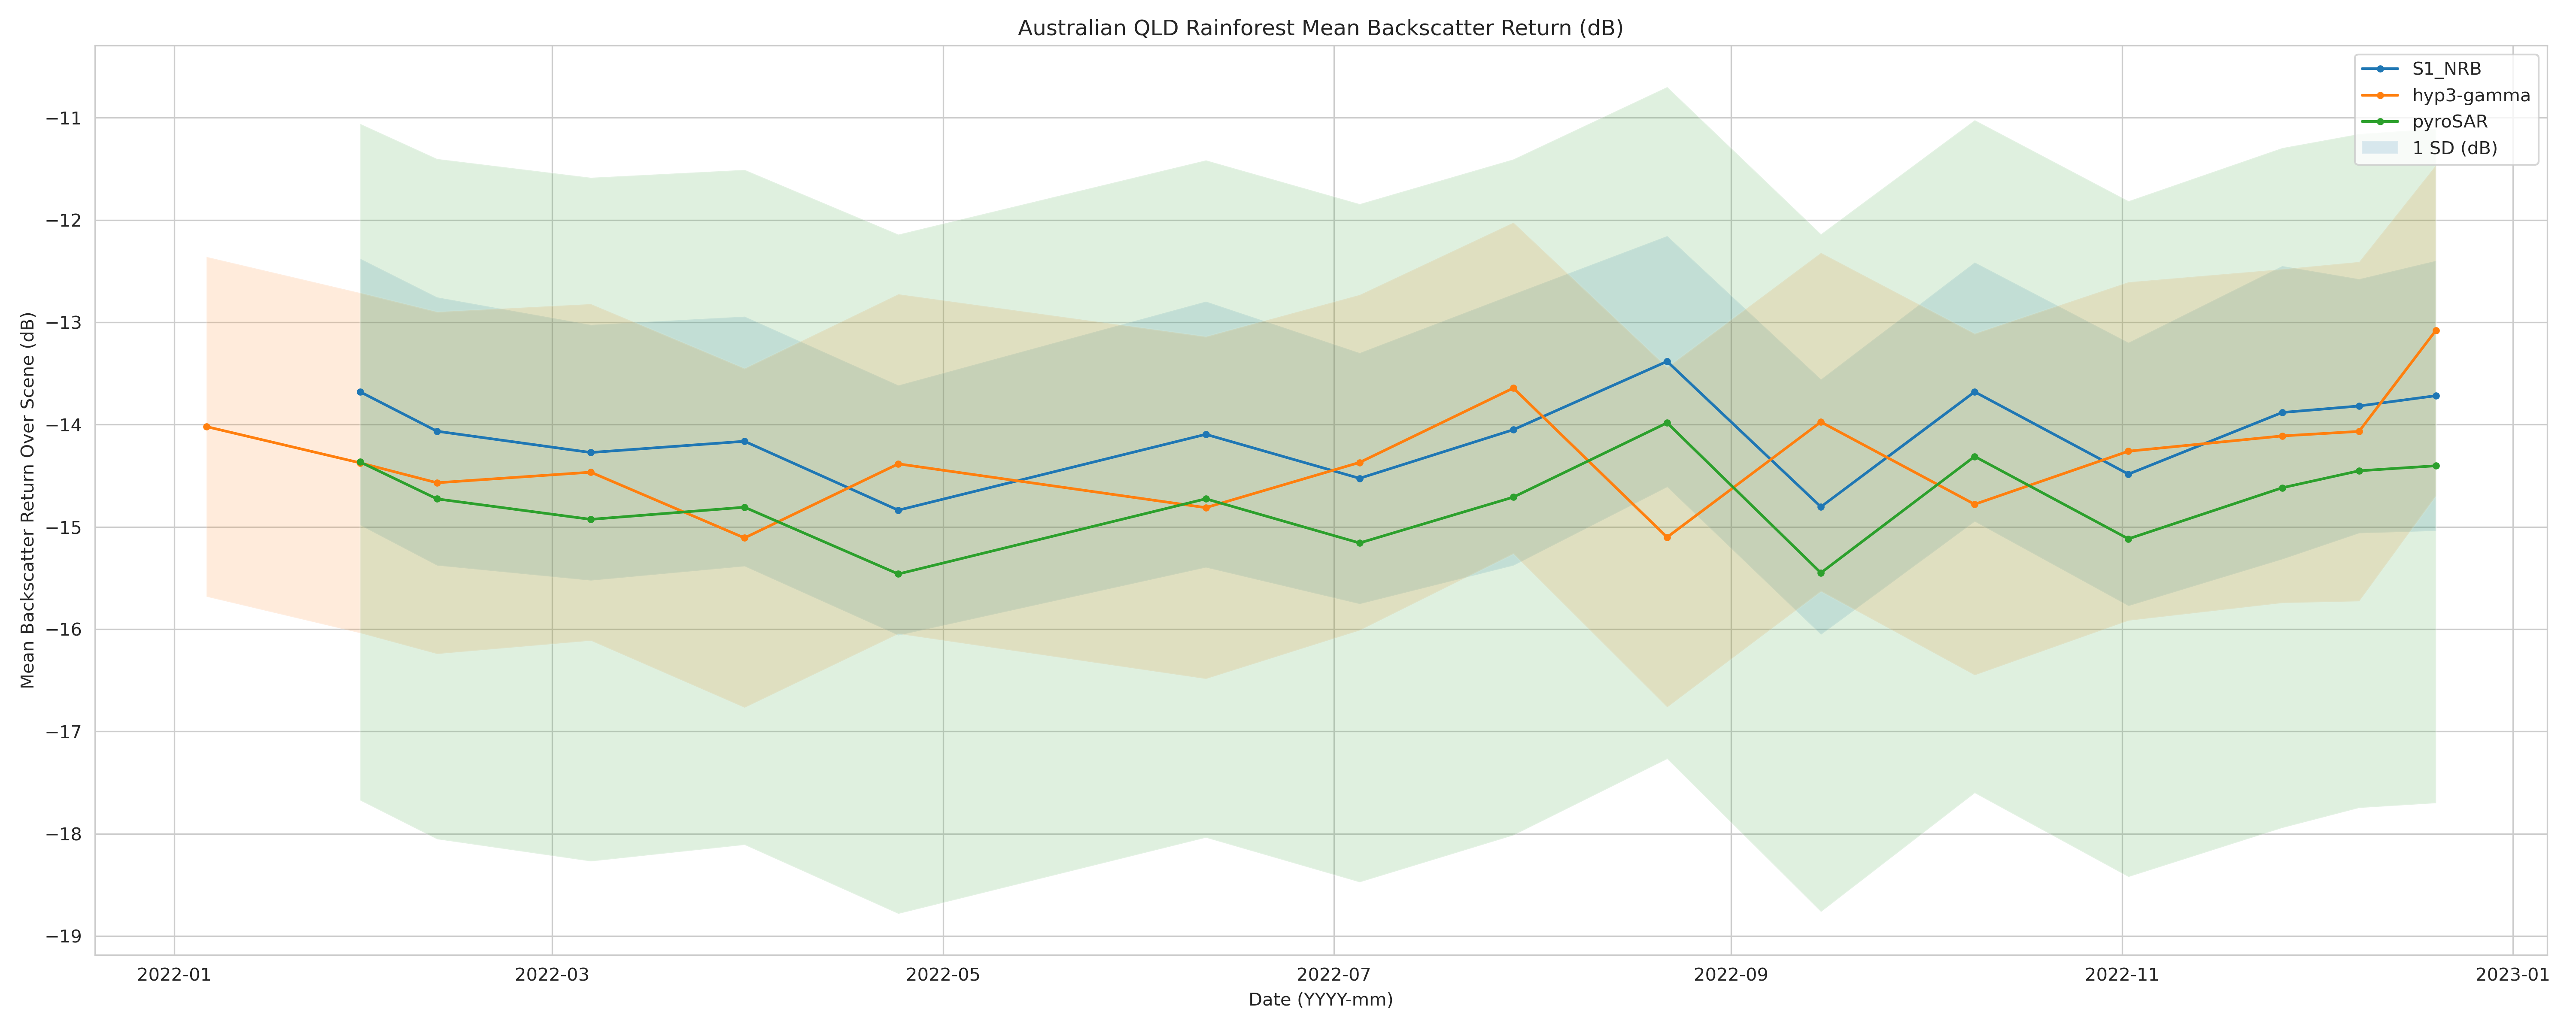
\includegraphics[width=0.9\textwidth]{rainforest_return.png}
\caption{\label{fig:rainforestvh} Mean (line plot) and standard deviation (shaded around the mean) VH backscatter return over time for the QLD rainforest test site. The values fall in the expected range of -15 to -12 dB literature.}
\end{figure}

\begin{figure}[ht]
\centering
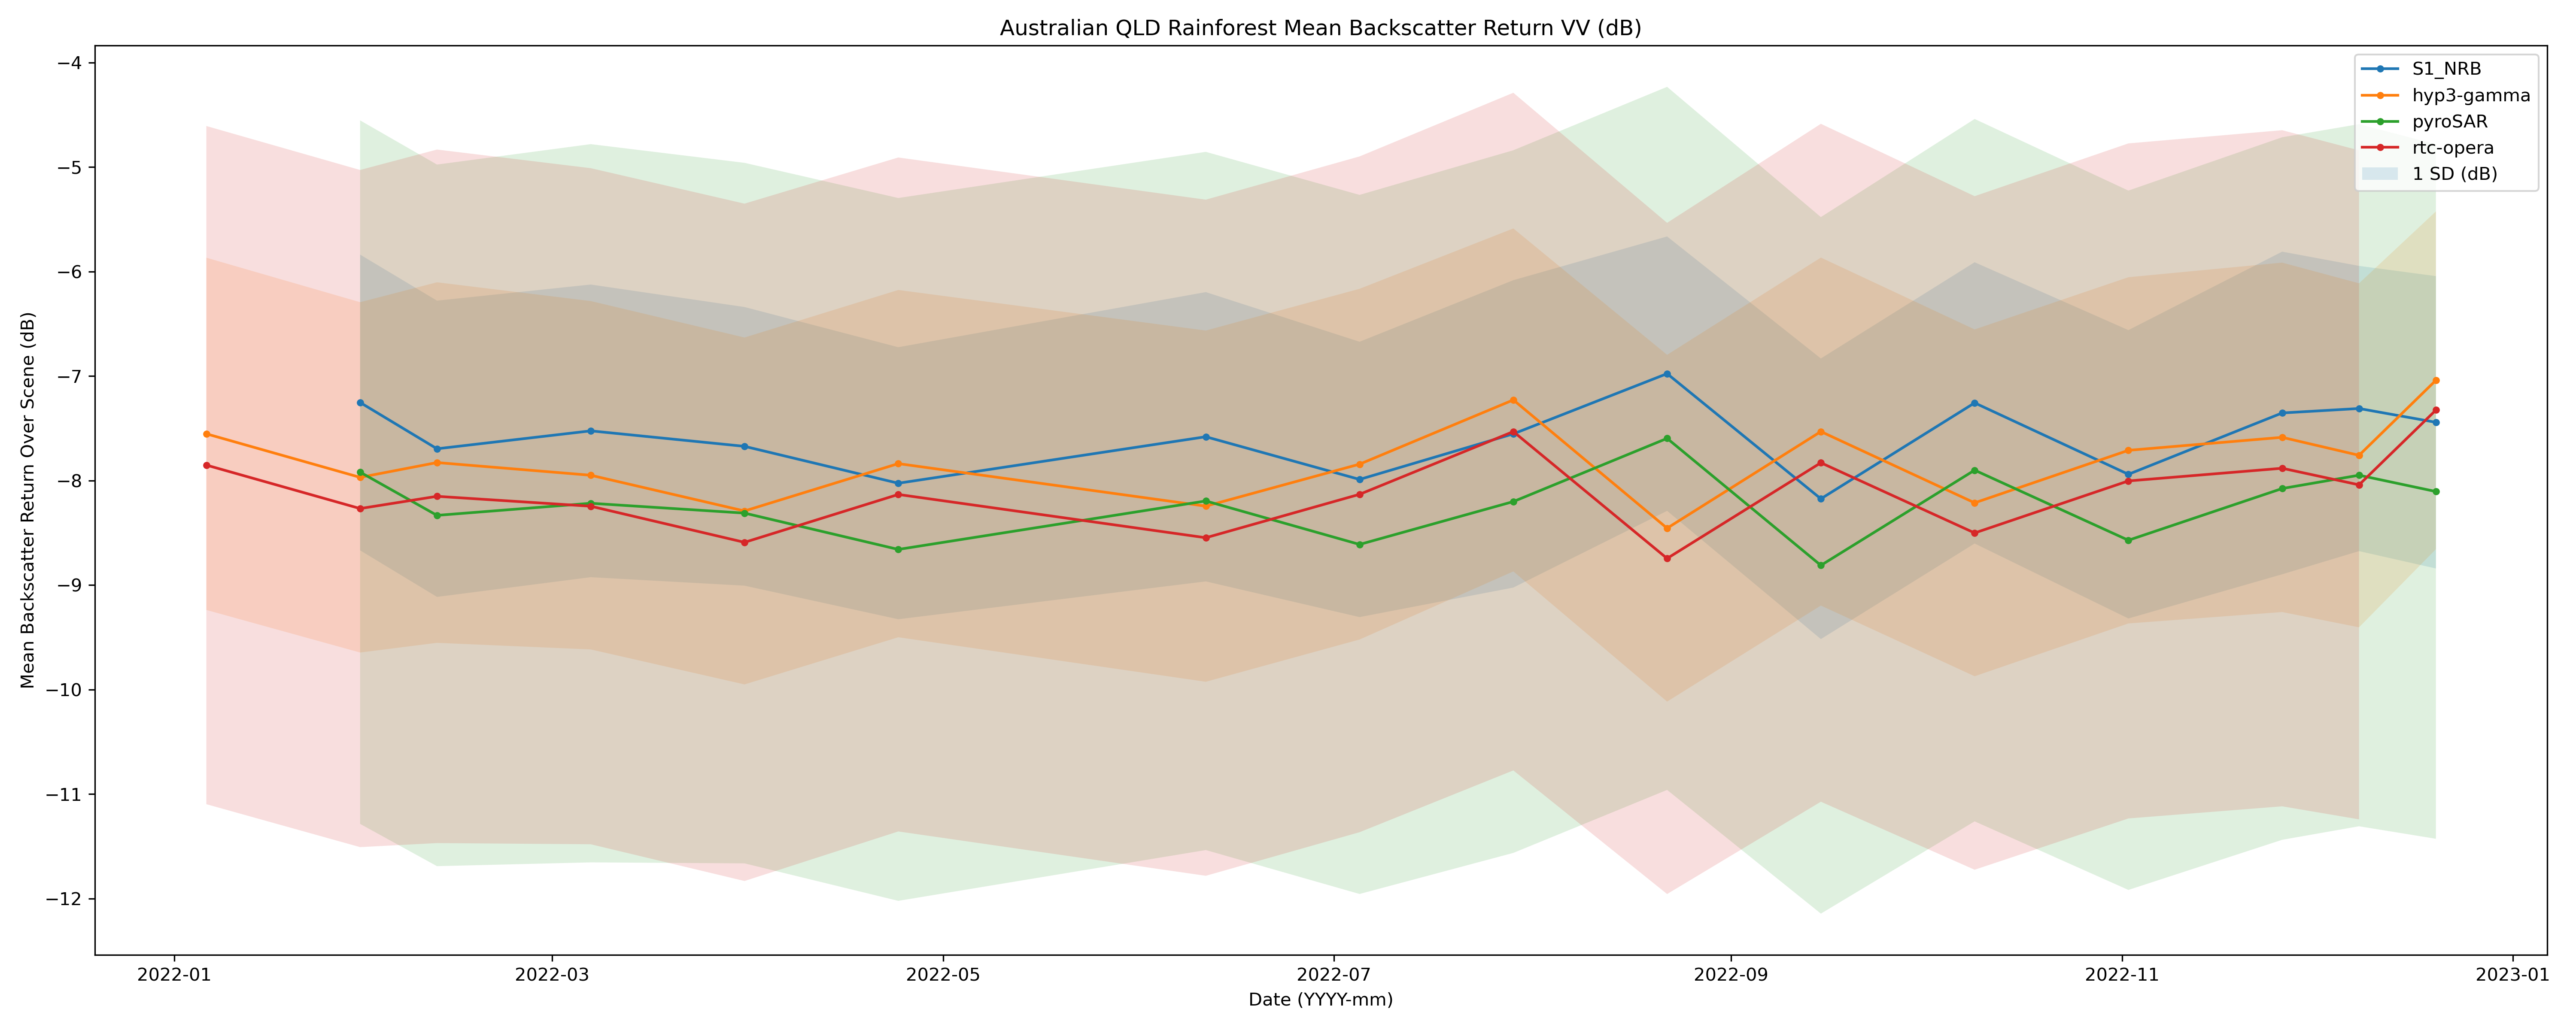
\includegraphics[width=0.9\textwidth]{rainforest_return_VV.png}
\caption{\label{fig:rainforestvv} Same as Figure \ref{fig:rainforestvh} for VV polarisation. The values fall in the expected range of -9 to -6 dB from literature.}
\end{figure}

\section{Geometric Quality}
\subsection{Incident Angle Gradient}

\begin{figure}[ht]
\centering
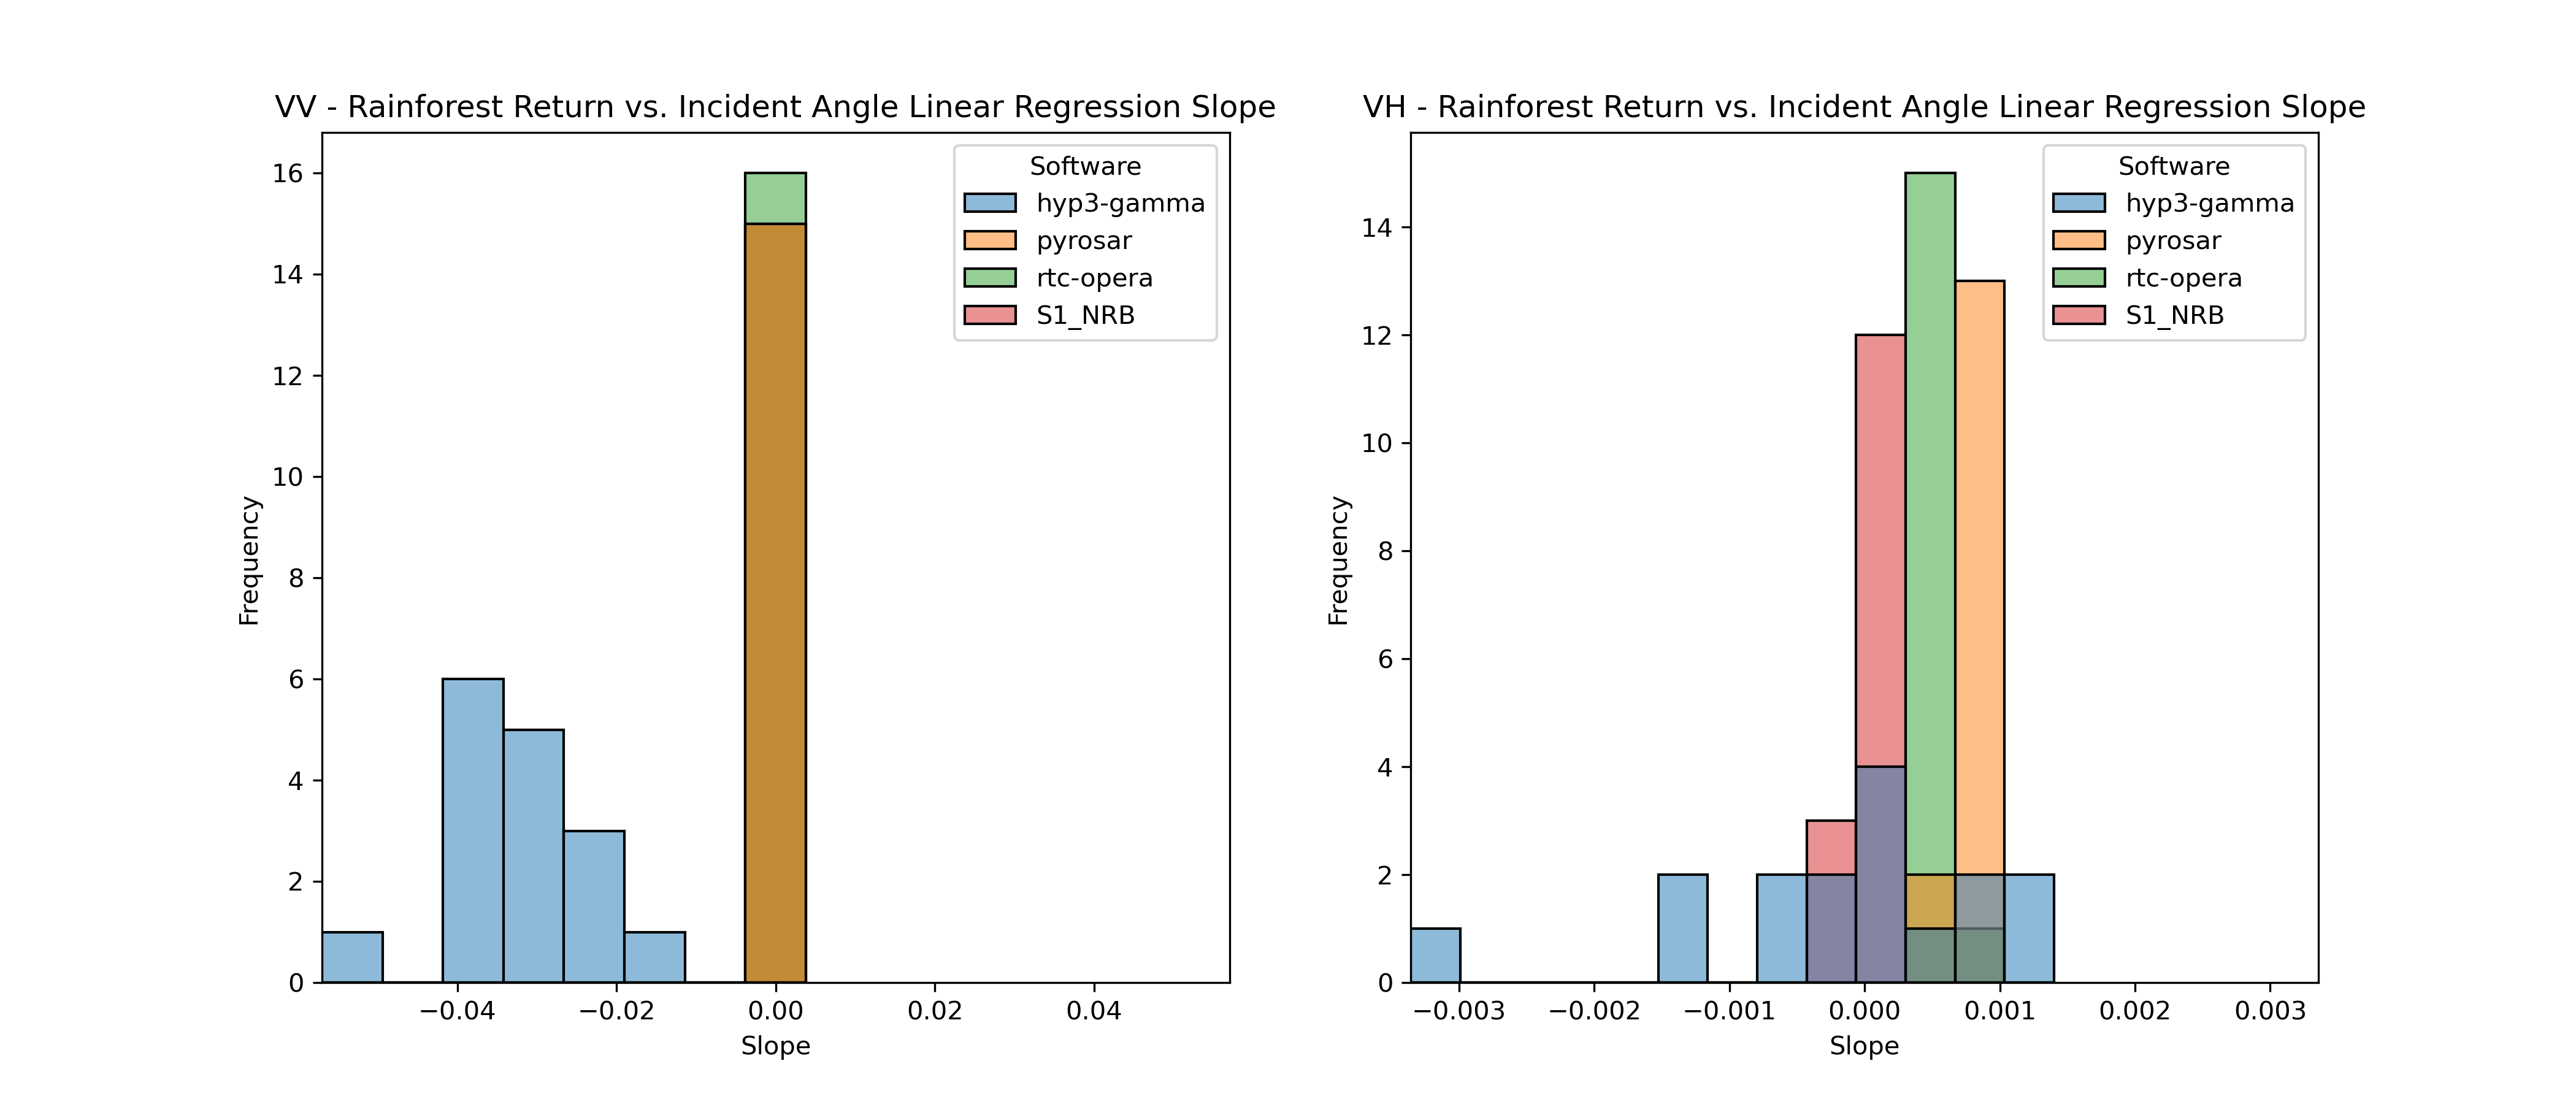
\includegraphics[width=\textwidth]{slope.png}
\caption{\label{fig:slope}}
\end{figure}

\begin{figure}[ht]
\centering
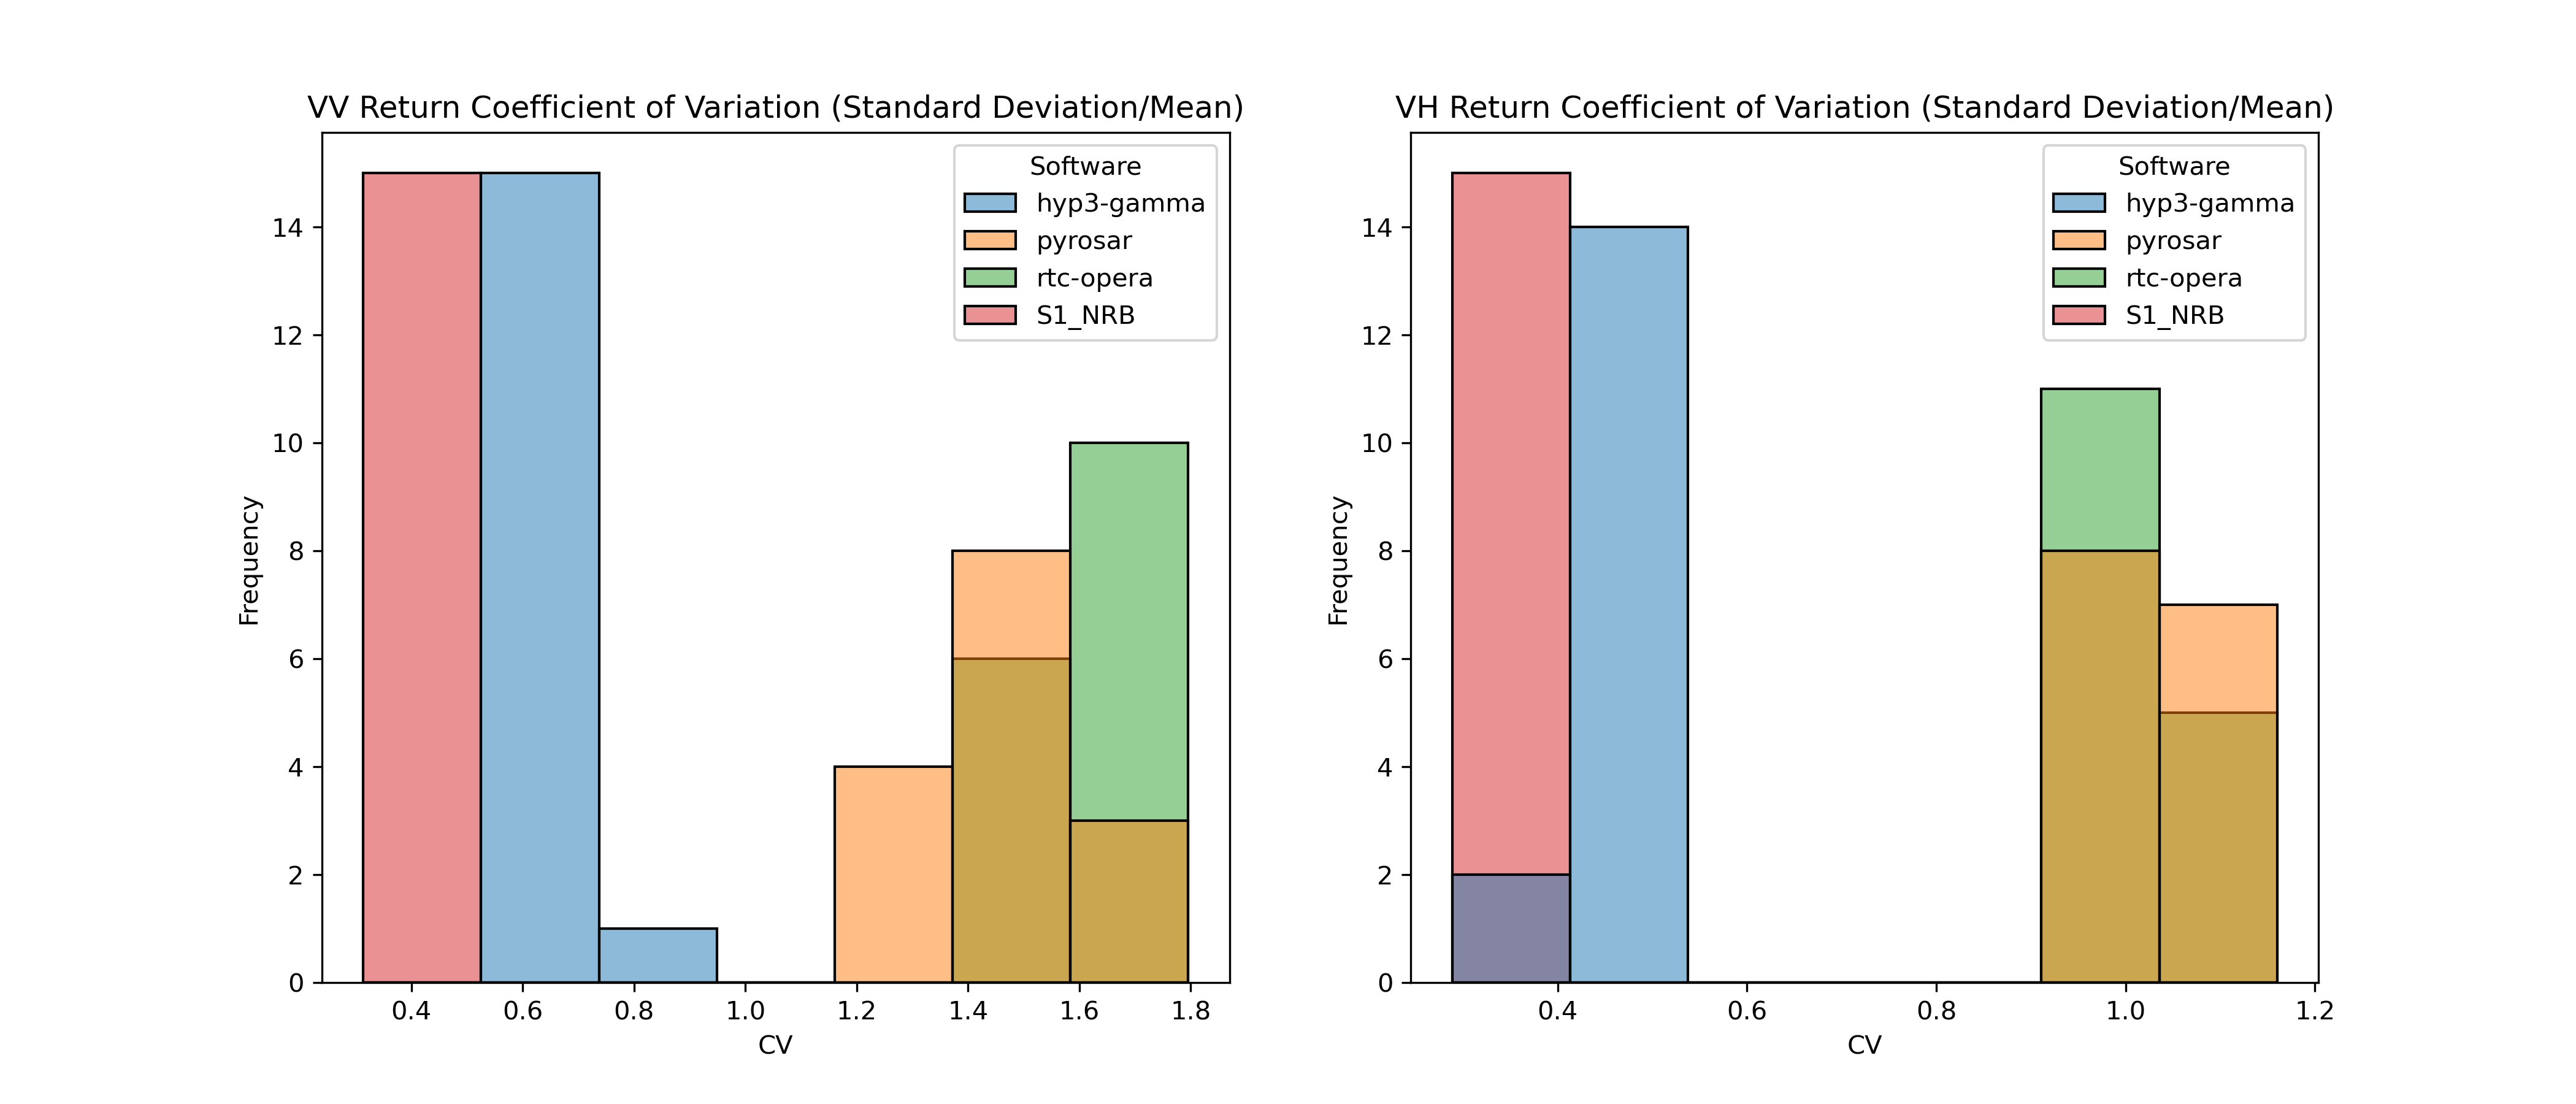
\includegraphics[width=\textwidth]{CV.png}
\caption{\label{fig:CV}}
\end{figure}

\section{Tabulated Summary of Results}

\begin{tabular}{lllrrr}
Software & Season & Polarisation & Mean (dB) & CV & Slope \\
\multirow[c]{8}{*}{S1-NRB} & \multirow[c]{2}{*}{Autumn} & VH & -13.85 & 0.30 & -3.67E-05 \\
 &  & VV & -7.37 & 0.36 & -7.27E-04 \\
 & \multirow[c]{2}{*}{Spring} & VH & -14.12 & 0.31 & -2.17E-05 \\
 &  & VV & -7.67 & 0.35 & -5.73E-04 \\
 & \multirow[c]{2}{*}{Summer} & VH & -14.12 & 0.30 & -4.58E-05 \\
 &  & VV & -7.62 & 0.34 & -6.55E-04 \\
 & \multirow[c]{2}{*}{Winter} & VH & -14.24 & 0.29 & -4.87E-05 \\
 &  & VV & -7.62 & 0.34 & -8.65E-04 \\
\multirow[c]{8}{*}{hyp3-gamma} & \multirow[c]{2}{*}{Autumn} & VH & -14.15 & 0.44 & -5.33E-04 \\
 &  & VV & -7.65 & 0.66 & -3.75E-02 \\
 & \multirow[c]{2}{*}{Spring} & VH & -14.45 & 0.45 & 9.29E-05 \\
 &  & VV & -7.97 & 0.68 & -3.03E-02 \\
 & \multirow[c]{2}{*}{Summer} & VH & -14.15 & 0.44 & 3.82E-04 \\
 &  & VV & -7.73 & 0.67 & -2.66E-02 \\
 & \multirow[c]{2}{*}{Winter} & VH & -14.52 & 0.45 & -8.61E-04 \\
 &  & VV & -7.89 & 0.66 & -4.12E-02 \\
\multirow[c]{8}{*}{pyrosar} & \multirow[c]{2}{*}{Autumn} & VH & -14.49 & 1.06 & 8.02E-04 \\
 &  & VV & -8.02 & 1.58 & 3.58E-03 \\
 & \multirow[c]{2}{*}{Spring} & VH & -14.80 & 1.00 & 7.54E-04 \\
 &  & VV & -8.33 & 1.37 & 3.30E-03 \\
 & \multirow[c]{2}{*}{Summer} & VH & -14.76 & 1.00 & 7.52E-04 \\
 &  & VV & -8.26 & 1.37 & 3.43E-03 \\
 & \multirow[c]{2}{*}{Winter} & VH & -14.87 & 1.09 & 7.33E-04 \\
 &  & VV & -8.26 & 1.60 & 3.35E-03 \\
\multirow[c]{8}{*}{rtc-opera} & \multirow[c]{2}{*}{Autumn} & VH & -14.42 & 0.99 & 6.13E-04 \\
 &  & VV & -7.95 & 1.55 & 2.59E-03 \\
 & \multirow[c]{2}{*}{Spring} & VH & -14.73 & 1.01 & 5.84E-04 \\
 &  & VV & -8.26 & 1.60 & 2.42E-03 \\
 & \multirow[c]{2}{*}{Summer} & VH & -14.42 & 1.00 & 6.21E-04 \\
 &  & VV & -8.02 & 1.60 & 2.67E-03 \\
 & \multirow[c]{2}{*}{Winter} & VH & -14.80 & 1.04 & 5.68E-04 \\
 &  & VV & -8.19 & 1.65 & 2.43E-03 \\
\end{tabular}

\subsection{How to add Citations and a References List}

You can simply upload a \verb|.bib| file containing your BibTeX entries, created with a tool such as JabRef. You can then cite entries from it, like this: \cite{greenwade93}. Just remember to specify a bibliography style, as well as the filename of the \verb|.bib|. You can find a \href{https://www.overleaf.com/help/97-how-to-include-a-bibliography-using-bibtex}{video tutorial here} to learn more about BibTeX.

If you have an \href{https://www.overleaf.com/user/subscription/plans}{upgraded account}, you can also import your Mendeley or Zotero library directly as a \verb|.bib| file, via the upload menu in the file-tree.

\subsection{Good luck!}

We hope you find Overleaf useful, and do take a look at our \href{https://www.overleaf.com/learn}{help library} for more tutorials and user guides! Please also let us know if you have any feedback using the Contact Us link at the bottom of the Overleaf menu --- or use the contact form at \url{https://www.overleaf.com/contact}.

\bibliographystyle{alpha}
\bibliography{sample}

\end{document}